\section{Problem Formulation}
\subsection{Mask Diffusion Models}
Diffusion models~\citep{ho2020denoising,song2021scorebased} contain a forward process that gradually corrupts data $\bm{x}_0\sim p_{data}(\bm{x}_0)$ into noisy variables $\bm{x}_{1:T}$ through $q(\bm{x}_{1:T}|\bm{x}_0)=\prod_{t=1}^{T}q(\bm{x}_t|\bm{x}_{t-1})$, and a backward process that models the joint probability as $p_{\theta}(\bm{x}_{0:T})=p_{\theta}(\bm{x}_T)\prod_{t=1}^Tp_{\theta}(\bm{x}_{t-1}|\bm{x}_t)$, denoising $\bm{x}_t$ to reconstruct $\bm{x}_0$. The parameters $\theta$ are learned by minimizing the negative log-likelihood via the evidence lower bound (ELBO):
\begin{align}
\label{eq:ori-loss-appen}
    -\log p_{\theta}(\bm{x}_0) & \leq \mathbb{E}_{q(\bm{x}_1|\bm{x}_0)}[-\log p_{\theta}(\bm{x}_0|\bm{x}_1)] + \KL(q(\bm{x}_T|\bm{x}_0)||p_{\theta}(\bm{x}_T))+\mathcal{L}_T, \\
    \label{eq:ori-loss-line2-appen}
    \text{with }
\mathcal{L}_T & =\sum_{t=2}^T\mathbb{E}_{q(\bm{x}_t|\bm{x}_0)}[\KL(q(\bm{x}_{t-1}|\bm{x}_t, \bm{x}_0)||p_{\theta}(\bm{x}_{t-1}|\bm{x}_t))].
\end{align}

\citet{hoogeboom2021argmax,austin2021structured} first proposed discrete diffusion models, where they define the forward process with a categorical distribution $q(\bm{x}_{t} \vert \bm{x}_{t-1})=\text{Cat}(\bm{x}_t;\bm{Q}_t^\top\bm{x}_{t-1})$, where $\bm{x}_t \in \{0, 1\}^K$ is a one-hot vector of vocabulary size $K$, and $\bm{Q}_t\in[0,1]^{K\times K}$ is the transition matrix. A special case is absorbing discrete diffusion, where $\bm{Q}_t=(1-\beta_t)I+\beta_t\mathbf{1}\bm{m}^\top$, with $\mathbf{1}$ being an all-ones vector of size $K$ and $\bm{m}$ the one-hot encoding of a special \mask token.
Starting from $\bm{x}_0$, the $t$-step marginal distribution is $q(\bm{x}_t|\bm{x}_0)=\text{Cat}(\bm{x}_t;\bm{p}=\bm{\overline{Q}}_t^\top\bm{x}_0)$, where the cumulative product is $\bm{\overline{Q}}_t = \prod_{i=1}^t\bm{Q}_i=\alpha_tI+(1-\alpha_t)\mathbf{1}\bm{m}^\top$, and $\alpha_t=\prod_{i=1}^t(1-\beta_t)$. We expect $\alpha_T$ to approach $0$ such that the fully noised data $\bm{x}_T$ equals $\bm{m}$ with probability $1$.

For any two arbitrary time points $0\leq s< t\leq 1$, the transition distribution between them is $q(\bm{x}_t|\bm{x}_s)=\text{Cat}(\bm{x}_t;\bm{\overline{Q}}_{s|t}^\top \bm{x}_s)$, where $\bm{\overline{Q}}_{s|t} = \bm{\overline{Q}}_s^{-1}\bm{\overline{Q}}_t=\frac{\alpha_t}{\alpha_s}I+(1-\frac{\alpha_t}{\alpha_s})\mathbf{1}\bm{m}^\top$. This allows us to compute the transition probability between any two timesteps using the ratio of their alpha values:
\begin{equation}
\label{eq:qxs-appen}
    q(\bm{x}_s|\bm{x}_t, \bm{x}_0) = \frac{q(\bm{x}_t|\bm{x}_s)q(\bm{x}_s|\bm{x}_0)}{q(\bm{x}_t|\bm{x}_0)}=
    \begin{cases}
        \frac{1\cdot(1-\alpha_s)}{1-\alpha_t} = \frac{1-\alpha_s}{1-\alpha_t} = 1- \frac{\alpha_s-\alpha_t}{1-\alpha_t} & \text{if } \bm{x}_t=\bm{x}_s=\bm{m}, \\
        \frac{(1-\frac{\alpha_t}{\alpha_s})\cdot\alpha_s}{1-\alpha_t} = \frac{\alpha_s-\alpha_t}{1-\alpha_t} & \text{if }\bm{x}_t=\bm{m}\neq \bm{x}_s. \\
    \end{cases}
\end{equation}
\begin{equation}
\label{eq:appen-px}
p_{\theta}(\bm{x_s}|\bm{x}_t)=\frac{\alpha_s-\alpha_t}{1-\alpha_t}f_{\theta}(\bm{x}_t)+\frac{1-\alpha_s}{1-\alpha_t}\bm{m}. 
\end{equation}
\begin{equation}
    \KL(q(\bm{x}_s|\bm{x}_t,\bm{x}_0)||p_{\theta}(\bm{x}_s||\bm{x}_t)) = 
    \begin{cases}
        \frac{\alpha_s-\alpha_t}{1-\alpha_t}\KL(\bm{x}_0||f_{\theta}(\bm{x}_t)), & \text{for } \bm{x}_t =\bm{m};\\
        0, & \text{for } \bm{x}_t \neq \bm{m}.\\
    \end{cases}
\end{equation}
Thus,
\begin{equation}
    \mathcal{L}_T = \sum_{t=2}^T [-\frac{\alpha_s-\alpha_t}{(t-s)(1-\alpha_t)}\delta_{\bm{x}_t,\bm{m}}\bm{x}_0^\top\log f_{\theta}(\bm{x}_t)\Delta_t].
\end{equation}
where $\delta_{\bm{x}_t,\bm{m}}$ is the indicator function, and $f_{\theta}(\bm{x}_t)$ represents the logits of the tokens.
In the continuous time limit where $T\rightarrow\infty$, we set a small timestep $\Delta_t=t-s=\frac{1}{T}\in(0,1)$. The sum over timesteps becomes an integral, and we have $\alpha_t^\prime=\frac{\alpha_t-\alpha_s}{t-s}$. Following the noise schedule $\alpha_t=1-t$, which is widely adopted by~\citet{shi2024simplified, sahoo2024simple, lou2023discrete, ou2024your}, we get $\frac{-\alpha_t^\prime}{1-\alpha_t}=\frac{1}{t}$.
This can be substituted into Eq.~(\ref{eq:ori-loss-line2-appen}), yielding the final ELBO at a sampled time $t$ as a weighted cross-entropy loss:
\begin{equation}
    \label{eq:dm-loss-appx}
    \mathcal{L}_{t} = \frac{1}{t}\mathbb{E}_{q(\bm{x}_t|\bm{x}_0)}\left[-\sum_{n=1}^N\delta_{\bm{x}_t^n,\bm{m}}(\bm{x}_0^{n})^\top\log f_{\theta}(\bm{x}_t)_n\right].
\end{equation}

\subsection{Generation Autoregressive-ness}
\label{appx:Causality}
We formally define local and global autoregressiveness (AR-ness) here.
\paragraph{Problem Setup}
Inference for dLLMs often utilizes low-confidence remasking with the number of diffusion timesteps set equal to the sequence length to ensure high performance.
In this setting, let the target sequence length be \(L\), and at each diffusion decoding iteration \(t=1,\dots,T\), the set of still-masked positions just before step \(t\) is
$M_{t-1}\subseteq\{1,2,\dots,L\}$.
We denote by \(p_t\in M_{t-1}\) the single position unmasked at step \(t\), thereby producing the full decoding order \(\{p_1,\dots,p_T\}\).

\paragraph{Local Autoregressive-ness: Contiguous Next-Token Prediction}
For any integer \(k\ge1\), define
\[
\mathbb{I}_{\mathrm{local}}(t,k)
=
\begin{cases}
1,&\text{if }\{p_{t-i}\}_{i=1}^k=\{\,p_t-i : i=1,\dots,k\},\\
0,&\text{otherwise.}
\end{cases}
\]
The \emph{Local AR-ness@\(k\)} is then computed as
$\mathrm{NTP@}k=\frac{1}{T}\sum_{t=1}^{T}\mathbb{I}_{\mathrm{local}}(t,k)$. Local AR-ness measures the tendency to decode the immediate successor of a previously generated token, capturing sequential continuity. It is non-increasing with \(k\), as it becomes harder to maintain longer consecutive spans.

\paragraph{Global Autoregressive-ness: Earliest-First Mask Selection}
At step \(t\), sort the masked positions $m_{t-1}^{(1)}<m_{t-1}^{(2)}<\cdots<m_{t-1}^{(|M_{t-1}|)}$.
Then
\[
\mathbb{I}_{\mathrm{global}}(t,k)
=
\begin{cases}
1,&\text{if }p_t\in\{m_{t-1}^{(1)},\dots,m_{t-1}^{(k)}\},\\
0,&\text{otherwise.}
\end{cases}
\]
The \emph{Global FMS-ratio@\(k\)} is
$\mathrm{FMS@}k=\frac{1}{T}\sum_{t=1}^{T}\mathbb{I}_{\mathrm{global}}(t,k)$. Global AR-ness measures the tendency to always unmask the earliest remaining token, capturing a front-to-back filling strategy. Together, these ratios reveal how the model behaves during generation. The ratio is non-decreasing with \(k\), as the criterion becomes easier to satisfy when more early positions are allowed.

\subsection{Coupled GRPO}
\label{appx:coupled-grpo}

In this section, we provide a detailed formulation of our Coupled GRPO algorithm. As discussed in \S\ref{sec:grpo}, we improve upon the baseline GRPO by introducing a coupled sampling scheme for more accurate probability estimation. The complete Coupled GRPO algorithm is presented in Algorithm~\ref{algo:coupled-grpo}.

\paragraph{Probability Estimation with Coupled Sampling}
For a given completion sequence $o$ of length $L$, we select $\lambda$ timestep pairs $(t, \hat{t})$ where $t + \hat{t} = T$. For each pair, we create two complementary masks $M_{t}$ and $M_{\hat{t}}$ defined as binary vectors in $\{0,1\}^{L}$, such that:
\begin{equation}
    \label{eq:complementary-masks}
    M_{t}\,\lor\,M_{\hat{t}}\;=\;\mathbf{1}, 
    \quad 
    M_{t}\,\land\,M_{\hat{t}}\;=\;\mathbf{0},
\end{equation}
where $\lor$ and $\land$ denote element-wise \texttt{OR} and \texttt{AND}, respectively, and $\mathbf{1}, \mathbf{0}\in\{0,1\}^{L}$ are the all-ones and all-zeros vectors.
The probability estimation for token $o^k$ (also marked as $\bm{x}_0$) is then computed as:
\begin{equation}
    \label{eq:coupled-prob}
    \pi_\theta(o^k| c,o_{t<T}^k) = \frac{1}{\lambda+1}\bigg[\sum_{t+\hat{t}=T}^{\lambda}[\mathcal{L}_{t}(\bm{x}_t) + \mathcal{L}_{\hat{t}}(\bm{x}_{\hat{t}})] + \mathcal{L}_{T}(\bm{x}_T)\bigg].
\end{equation}
$\mathcal{L}_{t}$ is the loss term from Eq~(\ref{eq:dm-loss-appx}) at timestep $t$. In detail, we have $\mathcal{L}_{t}(\bm{x}_t)=M_t\cdot \frac{1}{t}\cdot\text{CE}(\bm{x}_{t},\bm{x}_0)$ where CE stands for the cross entropy loss.

\begin{algorithm}[t]
\caption{Coupled GRPO: Policy Optimization with Coupled Sampling}
\begin{algorithmic}[1]
\State \textbf{Input:} Reference model $\pi_{ref}$, condition set $\mathcal{C}$, number of completions per condition $G$, code test cases $\mathcal{T}$, hyperparameters $\mu,\beta,\varepsilon$ and $\lambda=1$
\State Initialize $\pi_{\theta} \gets \pi_{ref}$
\While{not converged}
    \State update reference model $\pi_{ref} \gets \pi_{\theta}$
    \For{step $ = 1, \ldots, I$}
    \State $\pi_{old} \gets \pi_{\theta}$
    \State Sample a batch of condition $\mathcal{C}_b \sim \mathcal{C}$
    \State Sample $G$ completions $\{o_i\}_{i=1}^G \sim \pi_{old}(\cdot|c)$, for each $c \in \mathcal C_b$
    \State For each $o_i$, compute reward $r(o_i)$ by execute test cases $\mathcal T_c$ of each $c$
    \State Get advantage $\small A_i=r(o_i)-\frac1G\sum_{j=1}^G r(o_j)$ or LOO $\small A_i=r(o_i)-\frac1{G-1}\sum_{j\neq i}^G r(o_j)$
    \For{GRPO iteration $j = 1, \ldots, \mu$}
            \State Randomly sample a timestep pair $(t_j, \hat{t}_j)$ where $t_j + \hat{t}_j = T$
            \State Create complementary masks $M_{t_j}$ and $M_{\hat{t}_j}$ for batch
            \State Compute $\mathcal{L}_{t_j}$, $\mathcal{L}_{\hat{t}_j}$ and $\mathcal{L}_{T}$
            \State Compute coupled probability estimates in Eq~(\ref{eq:coupled-prob}) and importance ratios $\rho_i^k$
        \State Update $\pi_{\theta}$ by gradient descent on $\mathcal{J}_{\text{GRPO}}$ Eq~(\ref{eq:grpo-loss-cp})
    \EndFor
    \EndFor
\EndWhile
\State \Return $\pi_{\theta}$
\end{algorithmic}
\label{algo:coupled-grpo}
\end{algorithm}

\paragraph{Analysis}
The coupled sampling scheme provides several benefits:
(i) \textbf{Full Coverage}: Each token is guaranteed to be evaluated exactly once in each coupled pair, ensuring complete coverage of the sequence.
(ii) \textbf{Reduced Variance}: By evaluating each token under realistic partial-masking contexts, we reduce the variance in probability estimates compared to full masking.
(iii) \textbf{Computational Efficiency}: The coupled sampling requires only two additional forward passes per update compared to the d1~\citep{zhao2025d1} baseline when $\lambda=1$.
The variance reduction can be formally quantified in the next section, \S\ref{appx:coupled-grpo-theory}. 

{
  \subsection{Theoretical Analysis of Coupled-GRPO}
  \label{appx:coupled-grpo-theory}

  In this section, we provide a formal analysis of the coupled sampling scheme used to estimate the per-token log-probability proxies within our coupled-GRPO framework.
  GRPO requires stable estimates of these per-token quantities to compute the importance sampling ratios for the policy gradient update.
  We demonstrate that our coupled approach can be viewed as a direct and powerful application of the Antithetic Variates~\citep{hammersley1956new,hammersley1956general} variance reduction technique.
  We prove that it provides an unbiased estimator for the desired per-token quantity and, critically, that it is guaranteed to reduce estimation variance.
  
  
  The core challenge is to obtain a stable estimate of a score for each token in a generated sequence, where this score serves as a proxy for its log-probability. This score is defined as an expectation over a random process involving a diffusion timestep $t$ and a mask $M$.
  
  Assuming the linear noise schedule, the sampling process is as follows:
  A timestep $t$ is drawn from a distribution on $[0, 1]$, typically $t \sim U(0, 1)$.
  Different from \S\ref{appx:coupled-grpo} which formulates the loss computation batch-wise, in this section we examine the token-wise formulation.
  Conditional on $t$, a mask for each component in the sequence is sampled independently from a Bernoulli distribution $M_k \sim \text{Bernoulli}(t), k = 1, \dots, L$.

  For each token $k$ in a sequence $o$, we define a {per-token scoring function}, $g(t, M, k)$, which is non-zero only if token $k$ is masked:
  \begin{equation}
      g(t, M, k) = M_k \cdot \frac{1}{t} \cdot \ell(o^k | c, o_{\mathbf{1}-M}),
  \end{equation}
  where $\ell(\cdot)$ is the cross-entropy loss for token $o^k$ given the condition $c$ and the unmasked context $o_{\mathbf{1}-M}$. The quantity we wish to estimate for each token $k$ is its expected score:
  \begin{equation}
      v_k = \mathbb{E}_{t, M} [g(t, M, k)].
  \end{equation}
  This estimated $v_k$ is then used to compute the policy probability ratio $\pi_\theta/\pi_{\text{old}}$ in the GRPO objective.
  
  \subsubsection{Standard vs. Coupled Monte Carlo Estimators}
  
  
  \textbf{Standard MC Estimator.}~
  To estimate the vector of scores $(v_1, \dots, v_L)$, one can draw $2N$ i.i.d. pairs $\{(t_i, M_i)\}_{i=1}^{2N}$. The estimator for each token $k$ is:
  \begin{equation}
      \hat{v}_{k, \text{MC}} = \frac{1}{2N} \sum_{i=1}^{2N} g(t_i, M_i, k).
  \end{equation}
  In any given sample $i$, $g(t_i, M_i, k)$ is non-zero only for the subset of tokens $k$ where $M_{i,k}=1$. Many samples are needed to obtain a reliable, non-zero estimate for all tokens.
  
  \textbf{Coupled (Antithetic) Estimator.}~
  Our coupled sampling method generates antithetic pairs. We draw $N$ pairs $\{(t_i, M_i)\}_{i=1}^{N}$ and deterministically create their counterparts $(\hat{t}_i, \hat{M}_i) = (1-t_i, \mathbf{1}-M_i)$. The antithetic variates (AV) estimator for $v_k$ is:
  \begin{equation}
      \hat{v}_{k, \text{AV}} = \frac{1}{N} \sum_{i=1}^{N} \frac{g(t_i, M_i, k) + g(\hat{t}_i, \hat{M}_i, k)}{2}.
  \end{equation}
  A key structural property emerges here: for any given token $k$ and sample $i$, exactly one of the two terms in the inner sum is non-zero. This is because $M_{i,k}$ and $\hat{M}_{i,k} = 1 - M_{i,k}$ are binary complements. This guarantees that every token receives a non-zero score contribution from every coupled pair, ensuring full coverage and making the estimation process vastly more efficient.
  
  \subsubsection{Proofs}
  
  \textbf{Unbiasedness.}~
  We show that $\hat{v}_{k, \text{AV}}$ is an unbiased estimator of $v_k$.
  \begin{proof}
  The proof relies on showing that the joint probability distribution of $(t, M)$ is identical to that of its antithetic counterpart $(\hat{t}, \hat{M})$. 
  As proven in the previous version, under the symmetric sampling scheme for $t$ and the dependent Bernoulli sampling for $M$, we have $p(t,M) = p(\hat{t}, \hat{M})$.
  
  Since the random variables $(t,M)$ and $(\hat{t},\hat{M})$ are identically distributed, the expectation of any function of these variables is the same:
  \begin{equation}
      \mathbb{E}[g(t, M, k)] = \mathbb{E}[g(\hat{t}, \hat{M}, k)] = v_k.
  \end{equation}
  By linearity of expectation, the expectation of the AV estimator is:
  \begin{equation}
      \mathbb{E}[\hat{v}_{k, \text{AV}}] = \frac{1}{2N} \sum_{i=1}^{N} (\mathbb{E}[g(t_i, M_i, k)] + \mathbb{E}[g(\hat{t}_i, \hat{M}_i, k)]) = \frac{1}{2N} \sum_{i=1}^{N} (v_k + v_k) = v_k.
  \end{equation}
  Thus, the coupled estimator is unbiased.
  \end{proof}
  
  \paragraph{Variance Reduction.}~
  We now provide a direct and rigorous proof that the coupled estimator has lower variance than the standard MC estimator.
  \begin{proof}
  The variance of the AV estimator for token $k$ is given by:
  \begin{equation}
      \text{Var}(\hat{v}_{k, \text{AV}}) = \frac{\text{Var}(g(t, M, k)) + \text{Cov}(g(t, M, k), g(\hat{t}, \hat{M}, k))}{2N}.
  \end{equation}
  Variance is reduced if and only if the covariance term is negative.
  Let us analyze the covariance:
  \begin{equation}
      \text{Cov}(g(t, M, k), g(\hat{t}, \hat{M}, k)) = \mathbb{E}[g(t, M, k) \cdot g(\hat{t}, \hat{M}, k)] - \mathbb{E}[g(t, M, k)] \cdot \mathbb{E}[g(\hat{t}, \hat{M}, k)].
  \end{equation}
  Consider the product term inside the first expectation:
  \begin{equation}
      g(t, M, k) \cdot g(\hat{t}, \hat{M}, k) = \left( M_k \cdot \frac{1}{t} \ell(\dots) \right) \cdot \left( \hat{M}_k \cdot \frac{1}{\hat{t}} \ell(\dots) \right).
  \end{equation}
  The crucial insight is that the product of the mask indicators $M_k \cdot \hat{M}_k$ is always zero, since $\hat{M}_k = 1 - M_k$ and $M_k$ is either 0 or 1.
  % \begin{equation}
  %     M_k \cdot \hat{M}_k = M_k (1 - M_k) = M_k - M_k^2 = 0.
  % \end{equation}
  Therefore, the product of the scoring functions is identically zero for all possible values of $t$ and $M$. This means its expectation is also zero:
  \begin{equation}
      \mathbb{E}[g(t, M, k) \cdot g(\hat{t}, \hat{M}, k)] = 0.
  \end{equation}
  Substituting this back into the covariance formula:
  \begin{align}
      \text{Cov}(g(t, M, k), g(\hat{t}, \hat{M}, k)) &= 0 - (\mathbb{E}[g(t, M, k)]) \cdot (\mathbb{E}[g(\hat{t}, \hat{M}, k)]) \\
      &= -v_k \cdot v_k \\
      &= -v_k^2.
  \end{align}
  Since the loss $\ell(\cdot)$ is non-negative, the scoring function $g$ is non-negative. Its expectation, $v_k$, must therefore be non-negative. Assuming there is some configuration where a loss is incurred (i.e., $v_k > 0$), we have:
  \begin{equation}
      \text{Cov}(g(t, M, k), g(\hat{t}, \hat{M}, k)) = -v_k^2 < 0.
  \end{equation}
  The covariance is guaranteed to be negative. The variance reduction is therefore not just plausible but a mathematical certainty of this estimation scheme. The amount of reduction is:
  \begin{equation}
      \text{Var}(\hat{v}_{k, \text{MC}}) - \text{Var}(\hat{v}_{k, \text{AV}}) = \frac{\sigma^2_g}{2N} - \frac{\sigma^2_g - v_k^2}{2N} = \frac{v_k^2}{2N} > 0.
  \end{equation}
  \end{proof}
  This result stems directly from the mutually exclusive nature of the estimators for a given token within a coupled pair, a direct consequence of the complementary masks.
}

\section{Implementation Details}
\subsection{Training Details}
\label{appx:exp}
\paragraph{Adaptation pretraining}
During pre-training, we filter the code pre-training corpus from RefineCode~\citep{huang2024opencoder} and Stackv2~\citep{lozhkov2024starcoder}. Since RefineCode only provides each item's index in Stackv2, we built a local index engine to download the raw data from Stackv2. 
We also used text and math data from Fineweb~\citep{penedo2024finewebdatasetsdecantingweb} and DCLM-pro~\citep{zhou2024programming}. 
The final processed dataset contains around 400B tokens, as shown in Table~\ref{tab:training-data-recipes}. We adopted the code-to-text ratio suggested in Qwen-2.5-Coder~\citep{hui2024qwen2} and OpenCoder~\citep{huang2024opencoder}. 
The training was conducted on 10 nodes of 8 H100 GPUs each, using \texttt{BF16} and full-shard FSDP~\citep{zhao2023Fsdp}. The total wall-clock time for training on 65B tokens (100,000 global steps) was approximately 40 hours. 
The single-GPU batch size was $2$, and the context window was $4096$. Following LLaDA~\citep{nie2024scaling}, we truncated 1\% of the data to a random length to improve handling of variable-length inputs. 
Additionally, for another 1\% of the data, we used a random-length prefix as the condition during the diffusion process, which was kept unnoised. 
We used the Adam optimizer with a maximum learning rate of \texttt{2e-5}, with a linear warmup of 20,000 steps followed by a cosine decay schedule to 10\% of its peak value at the end of training. The attention mask annealing was performed over 10,000 steps, following DiffuLLaMA~\citep{gong2025scaling}. 
In our experiments, we observed that training on more tokens in Stage 1 did not improve performance on downstream tasks (Table~\ref{tab:fulltab}), nor did it lead to further improvements in Stage 2. 
Therefore, we used the model trained with 65B tokens as our Stage 1 model. With a higher-quality pre-training corpus, we might have reached different conclusions. 

\begin{table}[ht]
\centering
\begin{tabular}{@{} l l l l @{}} 
\toprule
\textbf{Source}                  & \textbf{\# tokens} & \textbf{Sample weight} & \textbf{Percentage} \\ 
\midrule
RefineCode from Stackv2 (code)        & 330B               & 1                      & 78\%               \\ 
Fineweb code page (text)     & 55B                & 1                      & \multirow{2}{*}{20\%} \\ 
DCLM subset  (text)      & 33B                & 1                      &                    \\ 
Fineweb math page (math)              & 3B                 & 3                      & 2\%                \\ 
\bottomrule
\end{tabular}
\caption{Adaptation Training Data Recipes on Stage 1}
\label{tab:training-data-recipes}
\end{table}

\begin{table}[t]
    \centering
    \small
    \setlength{\tabcolsep}{8pt} 
    \caption{Raw results on coding tasks for LLMs and dLLMs in 7/8B scale. $^*$ denotes that the results are collocated from public reports instead of evaluating by ourselves. BigCodeBench has completion (C) and instruction (I) version of template during evaluation. +SFT means we conduct the same instruction tuning with DiffuCoder-Instruct.}
    \begin{tabular}{@{} l cc cc cc cc @{}}
        \toprule
        \multirow{2}{*}{\textbf{Model}}
            & \multicolumn{2}{c}{HumanEval}
            & \multicolumn{2}{c}{MBPP}
            & \multicolumn{2}{c}{BigCodeBench (C)} 
            & \multicolumn{2}{c}{BigCodeBench (I)} \\
        \cmidrule(lr){2-3} \cmidrule(lr){4-5} \cmidrule(lr){6-7} \cmidrule(lr){8-9}
            & -   & Plus
            & -   & Plus
            & \multicolumn{1}{c}{Full} & \multicolumn{1}{c}{Hard}
            & \multicolumn{1}{c}{Full} & \multicolumn{1}{c}{Hard}\\
        \midrule
        \multicolumn{9}{c}{\textbf{Base Models}} \\
        \midrule
        \cellcolor{lightRed!12}Qwen2.5-Coder      & 61.6  & 51.8  & 75.9  & 61.4  & 46.1  & 16.2  & 40.2 & 14.2 \\
        \cellcolor{lightRed!12}OpenCoder$^*$      & 66.5  & 63.4  & 79.9  & 70.4  & 40.5  & 9.5  & – & – \\
        \cellcolor{lightYellow!12}LLaDA         & 35.4  & 30.5  & 50.1  & 42.1   & 18.9  & 4.1  & – & – \\
        \cellcolor{lightYellow!12}Dream         & 56.7  & 50.0  & 68.7  & 57.4    & 23.6  & 4.1  & – & –\\
        \cellcolor{lightYellow!12}DiffuCoder (Stage 2 65B)            & 67.1  & 60.4  & 74.2  & 60.9  & 40.2  & 12.8  & 1.8 & 0.7 \\
        \quad \cellcolor{lightYellow!5}- Stage 1 65B            & 39.0	& 31.7&	48.4&	38.3  & –  & –  & –  & – \\
        \quad \cellcolor{lightYellow!5}- Stage 1 720B            & 31.1	&23.3&	38.8&	31.3  & –  & –  & –  & – \\
        \quad \cellcolor{lightYellow!5}- Stage 2 16B            & 66.5	& 61.0	&71.9	&57.1&	36.7	&8.8  & –  & – \\
        \midrule
        \multicolumn{9}{c}{\textbf{Instruct Models}} \\
        \midrule
        \cellcolor{lightRed!12}Qwen2.5-Coder-Instruct & 90.2  & 85.4  & 83.9  & 72.0  & 50.7  & 21.6  & 42.2 & 18.2 \\
        \cellcolor{lightRed!12}Qwen2.5-Coder+SFT      
        & 82.9  
        & 75.6 
        & 80.1  
        & 66.1  
        & 46.9  
        & 16.2  
        & 39.5 & 14.9 \\
        \cellcolor{lightRed!12}OpenCoder-Instruct$^*$      
        & 83.5
        & 78.7
        & 79.1
        & 69.0
        & 40.3
        & 16.9
        & – & – \\
        \cellcolor{lightYellow!12}LLaDA-Instruct        
        & 35.4 
        & 31.7 
        & 31.5  
        & 28.6  
        & 16.5  
        & 2.7  
        & 14.1 & 1.4 \\
    \cellcolor{lightYellow!12}Dream-Instruct        
        & 57.9  
        & 53.7  
        & 68.3  
        & 56.1 
        & 10.6
        & 0.7 
        & 11.4 & 2.7 \\
    \cellcolor{lightYellow!12}Dream+SFT
        & 56.7  
        & 50.6  
        & 71.7  
        & 58.7 
        & 27.4
        & 6.1 
        & 25.9 & 5.4 \\
    \cellcolor{lightYellow!12}DiffuCoder-Instruct (5 ep)  
        & 72.0
        & 65.2
        & 75.1 
        & 61.9  
        & 35.7 
        & 12.2  
        & 34.0 & 8.8 \\
        \quad \cellcolor{lightYellow!5}- 1 epoch            & 67.1	& 60.4	& 75.7&	61.9	&31.1	&8.1&	32.0&	6.1 \\
        \quad \cellcolor{lightYellow!5}- 1 ep flexible padding            & 65.2&	58.5&	71.2&	59.5	&35.4	&11.5&	32.4	&10.1 \\
        \cellcolor{lightYellow!12}\quad + coupledGRPO (1ep)&73.2	&68.3	&78.6&	67.5	&40.4&	10.8	&37.5&	10.8\\
        \cellcolor{lightYellow!5}\quad + coupledGRPO (2ep)&70.1	&65.2	&79.1&	65.3&	42.8&	14.9&39.4	&13.5\\
        \midrule
        \multicolumn{9}{c}{\textbf{Commercial Models}} \\
        \midrule
        \cellcolor{lightRed!12}GPT 4o$^*$             & 90.2  & –     & 82.2  & –     & 49.9  & –   & –  &–\\
        \cellcolor{lightYellow!12}Mercury$^*$             & 90.0    & –     & 77.1  & –      & 45.5  & –   &– &– \\
        \cellcolor{lightYellow!12}Gemini Diffusion$^*$            & 89.6    & –     & 76.0  & –       & 45.4  & –   & – & –\\
        \bottomrule
    \end{tabular}
    \label{tab:fulltab}
\end{table}


\paragraph{Mid-training}
We used around 16B tokens of annealing code data~\citep{huang2024opencoder} during mid-training. This dataset contains an algorithmic corpus and synthetic data, such as high-quality code snippets and code textbooks. 
This high-quality mid-training data significantly improves the capacity of the base model, and we chose the model trained on 65B tokens (roughly 4 epochs over the training data) as the final version of DiffuCoder Base. 
The training was carried out on 8 nodes with 8 A100 GPUs each, using \texttt{BF16} and full-shard FSDP~\citep{zhao2023Fsdp}, which took 90 hours of wall-clock time. We used the Adam optimizer with a maximum learning rate of \texttt{1e-5} and a linear warmup of 2,000 steps. 
Other settings were the same as in Stage 1.
\paragraph{Instruction tuning}
We conducted classifier-free guidance SFT~\citep{gong-etal-2023-diffuseq, nie2024scaling, ye2024diffusion} for DiffuCoder using 436K instruction tuning samples from OpenCoder~\citep{huang2024opencoder}. 
The classifier-free guidance approach uses a conditional mask to prevent the diffusion process from adding noise to the condition prefix. We used the same chat template as Qwen2.5-Coder~\citep{hui2024qwen2}. 
We trained a new padding token that was used to pack each sample to a fixed length to control the generation length. We compared different SFT strategies for DiffuCoder instruction tuning, including: (i) using a fixed sequence length of 2048 for each sample with a conditional mask; (ii) using a fixed 2048 length but mixing conditional and unconditional training; and (iii) \emph{flexible padding}, where we padded to the maximum sequence length in the current batch instead of a fixed 2048. Finally, we progressively added a conditional mask for the first epoch, considering that Stages 1 and 2 were trained unconditionally, and then trained the remaining 4 epochs using a fixed sequence length of 2048. The SFT code is based on LLaMA-Factory\footnote{\url{https://github.com/hiyouga/LLaMA-Factory}}. The training was performed on 8 nodes of 8 H100 GPUs each, using \texttt{BF16} and ZeRO2~\citep{rajbhandari2020zero}, taking around 24 hours. 
We used the Adam optimizer with a maximum learning rate of \texttt{1e-5} and a linear warmup ratio of 0.1, followed by a cosine decay schedule to 10\% of its peak value at the end of training.
\paragraph{Coupled GRPO}
For RL training, for both our model and the ablation baselines, we filtered 21K hard samples from Acecoder-87k~\citep{zeng2025acecoder} with verifiable test cases and trained for one epoch. 
We used the pass rate of reference solutions in this dataset to filter for questions with a low average (bottom 20\%) and high variance (top 40\%) pass rate. These were marked as hard samples, yielding the final 21K samples used for GRPO training. 
We found that filtering the training samples by difficulty into a proper range is important. We used the online sandbox E2B\footnote{\url{https://e2b.dev/}} for code execution and reward verification. 
We trained the models on a single node with 8 H100 GPUs for a wall-clock time of 40 hours.
The default GRPO training parameters were: reference model sync steps $64$, number of iterations $\mu= 2$, $\beta=0.01$, $ \varepsilon=0.5$, learning rate \texttt{1e-6}, and maximum completion length $256$. The rollout parameters were: diffusion timesteps $256$, rollout samples $G=10$, and sampling temperature $1.2$. 
When sampling coupled $t$, we empirically chose a range of $[0.2, 0.8]$ instead of $[0, 1.0]$ to avoid extreme loss values (Figure~\ref{fig:unw-loss-curve}). 
Despite training for only one epoch with coupled GRPO, we observed that DiffuCoder-Instruct's performance continued to rise as we added more training steps.

\begin{figure}[h]
    \centering
    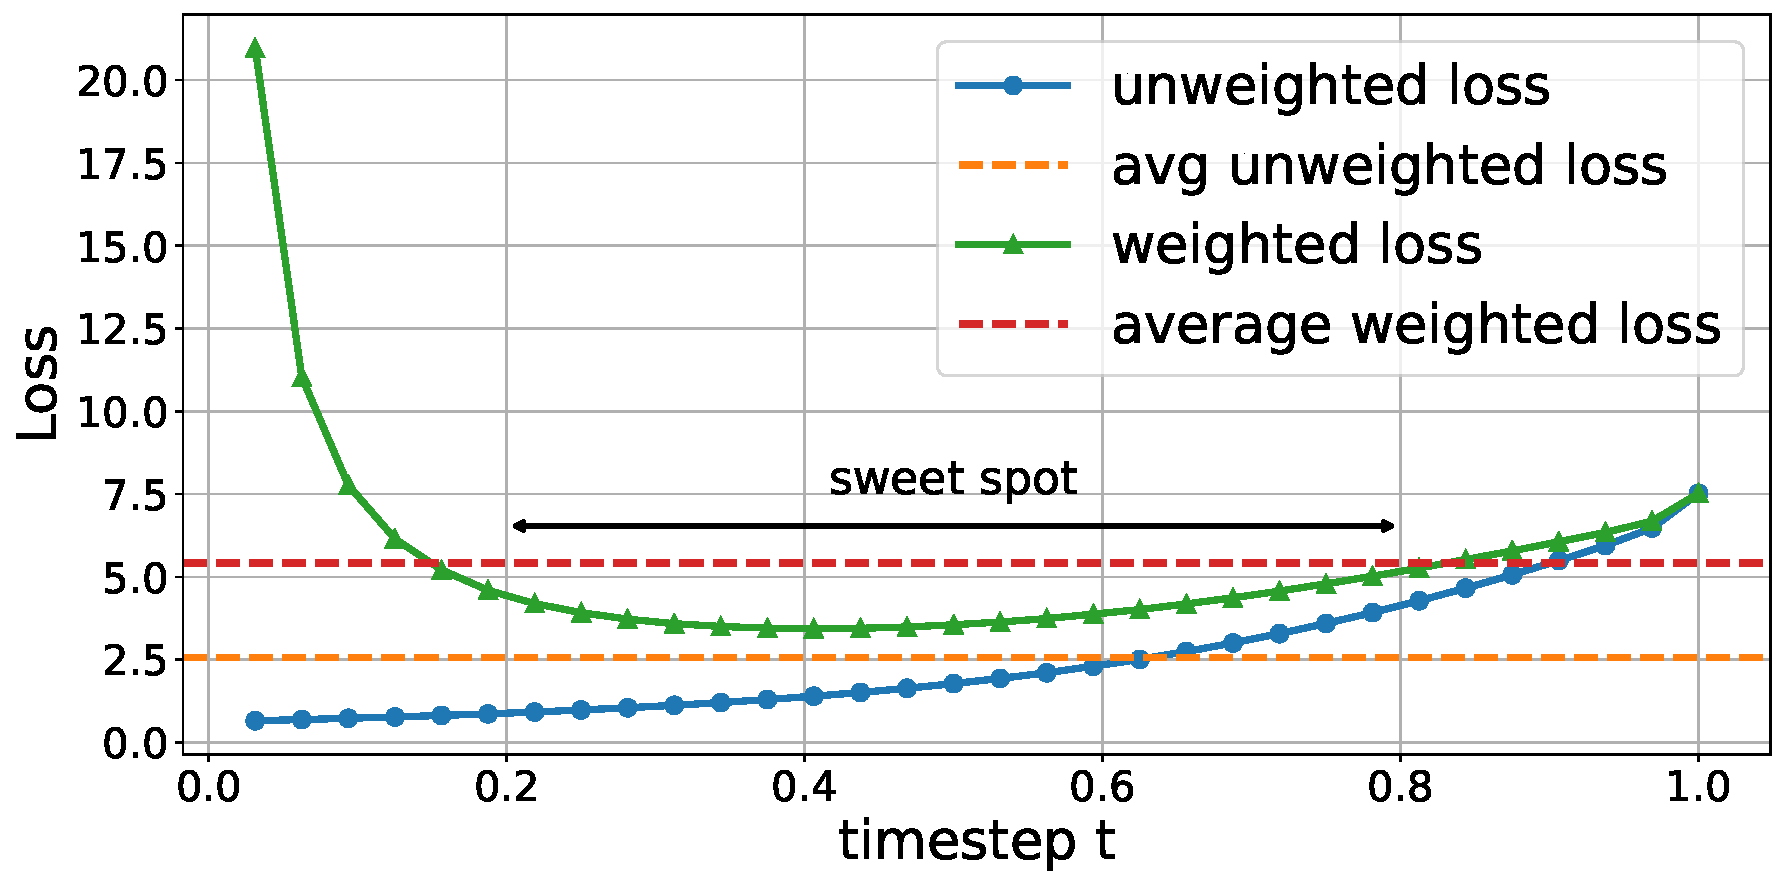
\includegraphics[width=0.5\linewidth]{fig/unw-loss-curve.pdf}
    \caption{Validation loss distribution of DiffuLLaMA~\citep{gong2025scaling} for different timesteps. The weighted loss refers to $\mathcal L_t$ in Eq.~(\ref{eq:dm-loss-appx}), while the unweighted loss refers to the cross-entropy term in the masked diffusion loss without the $1/t$ weighting. Timesteps that are too large or too small will lead to extreme values. The sweet spot is in the span of $[0.2, 0.8]$, which is also consistent for DiffuCoder.}
    \label{fig:unw-loss-curve}
\end{figure}

We designed a weighted reward for each completion $o_i$ as $r(o_i) = 2.0 \times r_{\text{code}}(o_i) + 0.5 \times r_{\text{format}}(o_i)$.
$r_{\text{code}}(o_i)$ is the pass rate on the test cases, evaluated only if $r_{\text{format}}(o_i) = 1$.
\begin{itemize}
    \item 0.5 if $o_i$ contains a valid Markdown code block and passes a Python syntax check;
    \item 0.25 if the code block format is correct but the code has a syntax error;
    \item 0 if the Markdown block format is not matched.
\end{itemize}


The raw results are in Table~\ref{tab:fulltab}. Our design choices in \S\ref{appx:exp} rely on these results. DiffuCoder Base underperforms on the instruction-query BigCodeBench (I), likely because the pre-training corpus teaches the base model to focus on completion rather than instruction following. 
Consequently, it fares better on the subset BigCodeBench (C) with completion query. After instruction tuning, DiffuCoder-Instruct achieves reasonable performance on BigCodeBench (I), indicating that instruction tuning teaches the model to follow instructions.
% Requires: \usepackage{tcolorbox,caption}
\begin{table}[h]
    \centering
    \begin{minipage}[t]{0.48\textwidth}
        \captionsetup{width=\linewidth}
        \caption{Chat template during the evaluation for HumanEval and BigCodeBench (C).}
        \label{tab:temp1}
        \centering
        \begin{tcolorbox}[
            colback=gray!10,
            boxrule=0.5pt,
            left=2mm,right=2mm,
            top=2mm,bottom=2mm,
            width=\linewidth,
        ]
{\ttfamily\small
<|im\_start|>system\\
You are a helpful assistant.<|im\_end|>\\
<|im\_start|>user\\
Please complete the following problem:\\
```\\
\{prompt\}\\
```\\
<|im\_end|>\\
<|im\_start|>assistant\\
Here is the code to solve this problem:\\
```python
}
        \end{tcolorbox}
    \end{minipage}\hfill
    \begin{minipage}[t]{0.48\textwidth}
        \captionsetup{width=\linewidth}
        \caption{Chat template during the evaluation for MBPP and BigCodeBench (I).}
        \label{tab:temp2}
        \centering
        \begin{tcolorbox}[
            colback=gray!10,
            boxrule=0.5pt,
            left=2mm,right=2mm,
            top=2mm,bottom=2mm,
            width=\linewidth,
        ]
{\ttfamily\small
<|im\_start|>system\\
You are a helpful assistant.<|im\_end|>\\
<|im\_start|>user\\
```\\
\{prompt\}\\
```\\
<|im\_end|>\\
<|im\_start|>assistant\\
Here is the code to solve this problem:\\
```python
}
        \end{tcolorbox}
    \end{minipage}
\end{table}

\subsection{Evaluation Details}
By default, LLaDA~\citep{nie2024scaling} employs low confidence remasking with temperature $0$, while Dream~\citep{dream2025} uses top negative entropy remasking with temperature $0.2$. 
Both models use a maximum sequence length and diffusion timesteps of $512$. GSM8K tests are conducted using lm-harness\footnote{\url{https://github.com/EleutherAI/lm-evaluation-harness}}, and code benchmarks are based on Qwen2.5-Coder's evaluation suitcase\footnote{\url{https://github.com/QwenLM/Qwen2.5-Coder/tree/main/qwencoder-eval}}. 
DiffuCoder shares the architecture (Qwen2.5-7B), tokenizer, and inference implementation of Dream-7B. The chat templates we used during the inference are listed below.

\section{Additional Results}
\subsection{Entropy Pattern}
In \S\ref{sec:analysis}, we present the phenomenon \emph{entropy sink} and illustrate the L-shaped distribution of the confidence score for a single time step (the first forward). In Figure~\ref{fig:appx-entropy}, we extend the visualization to 2D heatmaps. We can still observe a casual bias in these examples, but more token information and flexibility are involved compared to the strict causal mask.
\label{sec:appx:entropy}
\begin{figure}[ht]
  \centering
  \begin{subfigure}[c]{0.32\textwidth}
    \centering
    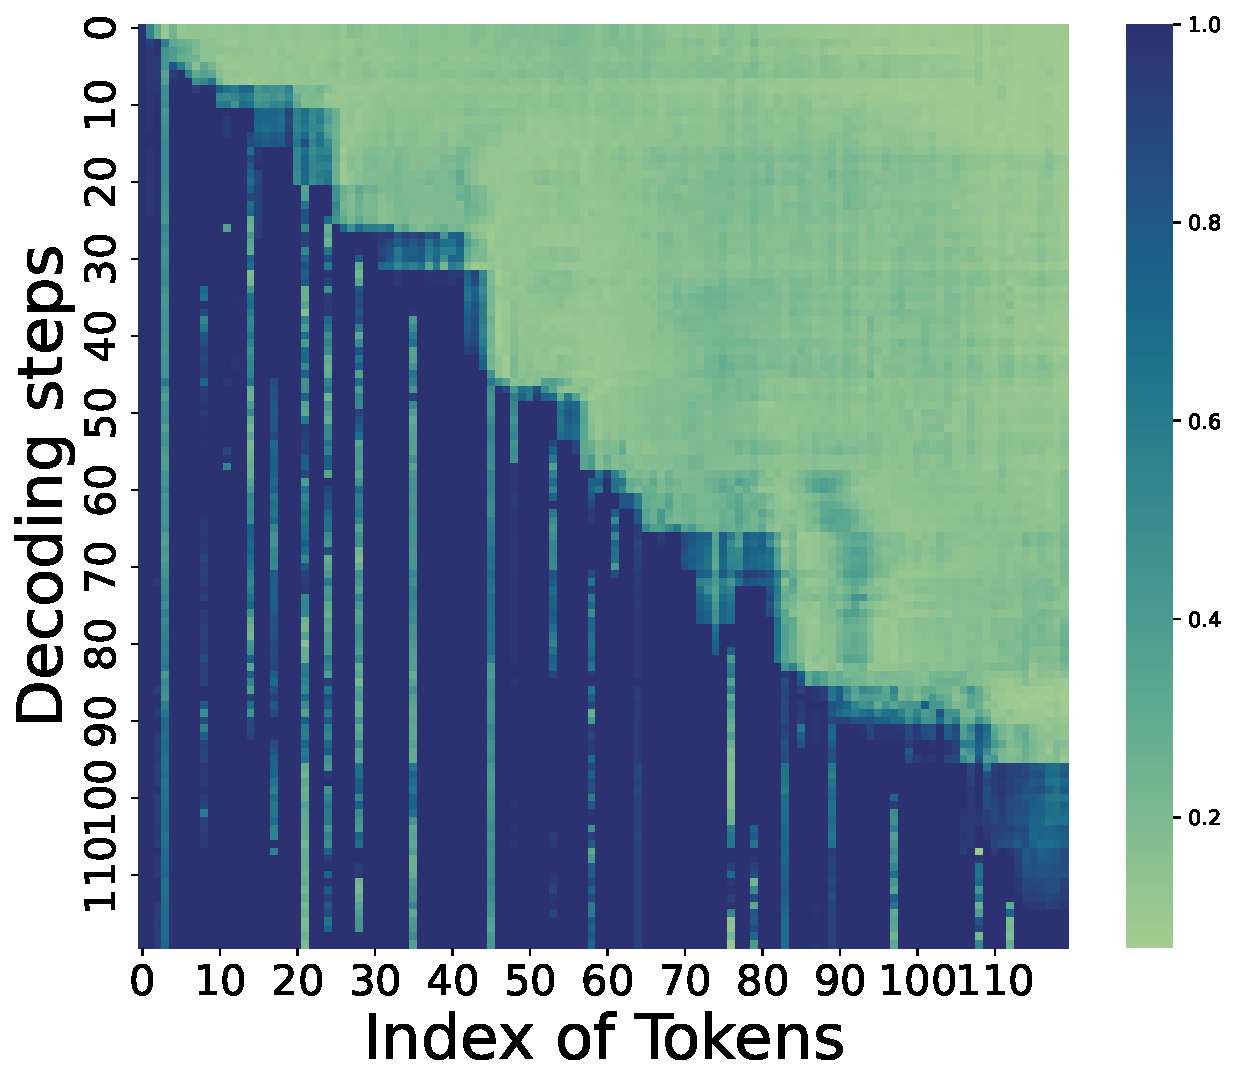
\includegraphics[width=\linewidth]{fig/heatmap.pdf}
  \end{subfigure}
  \hfill
  \begin{subfigure}[c]{0.32\textwidth}
    \centering
    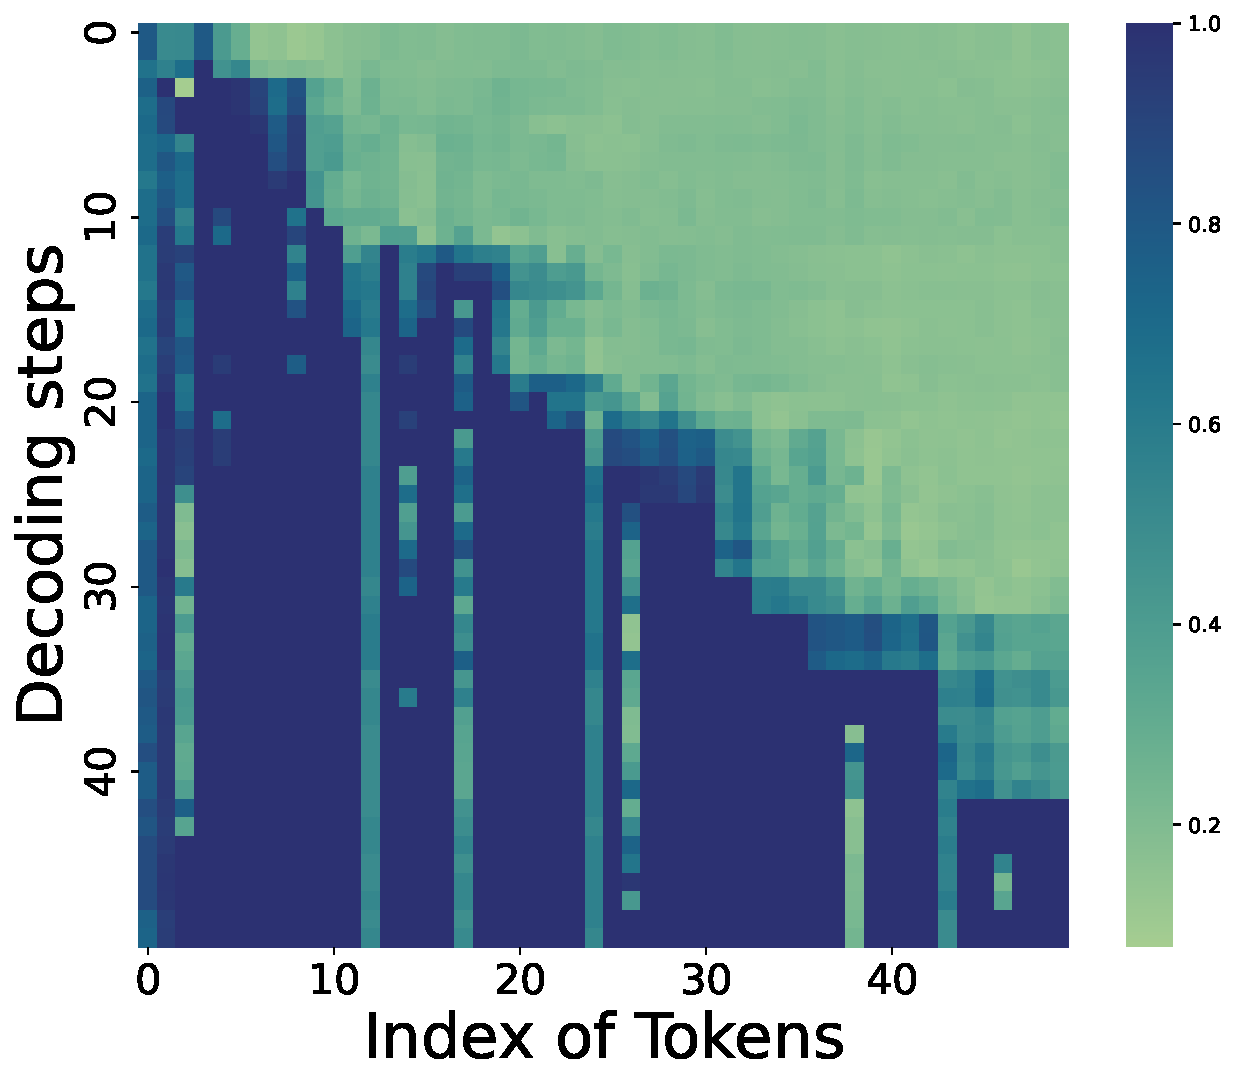
\includegraphics[width=\linewidth]{fig/heatmap2.pdf}
  \end{subfigure}
  \hfill
  \begin{subfigure}[c]{0.32\textwidth}
    \centering
    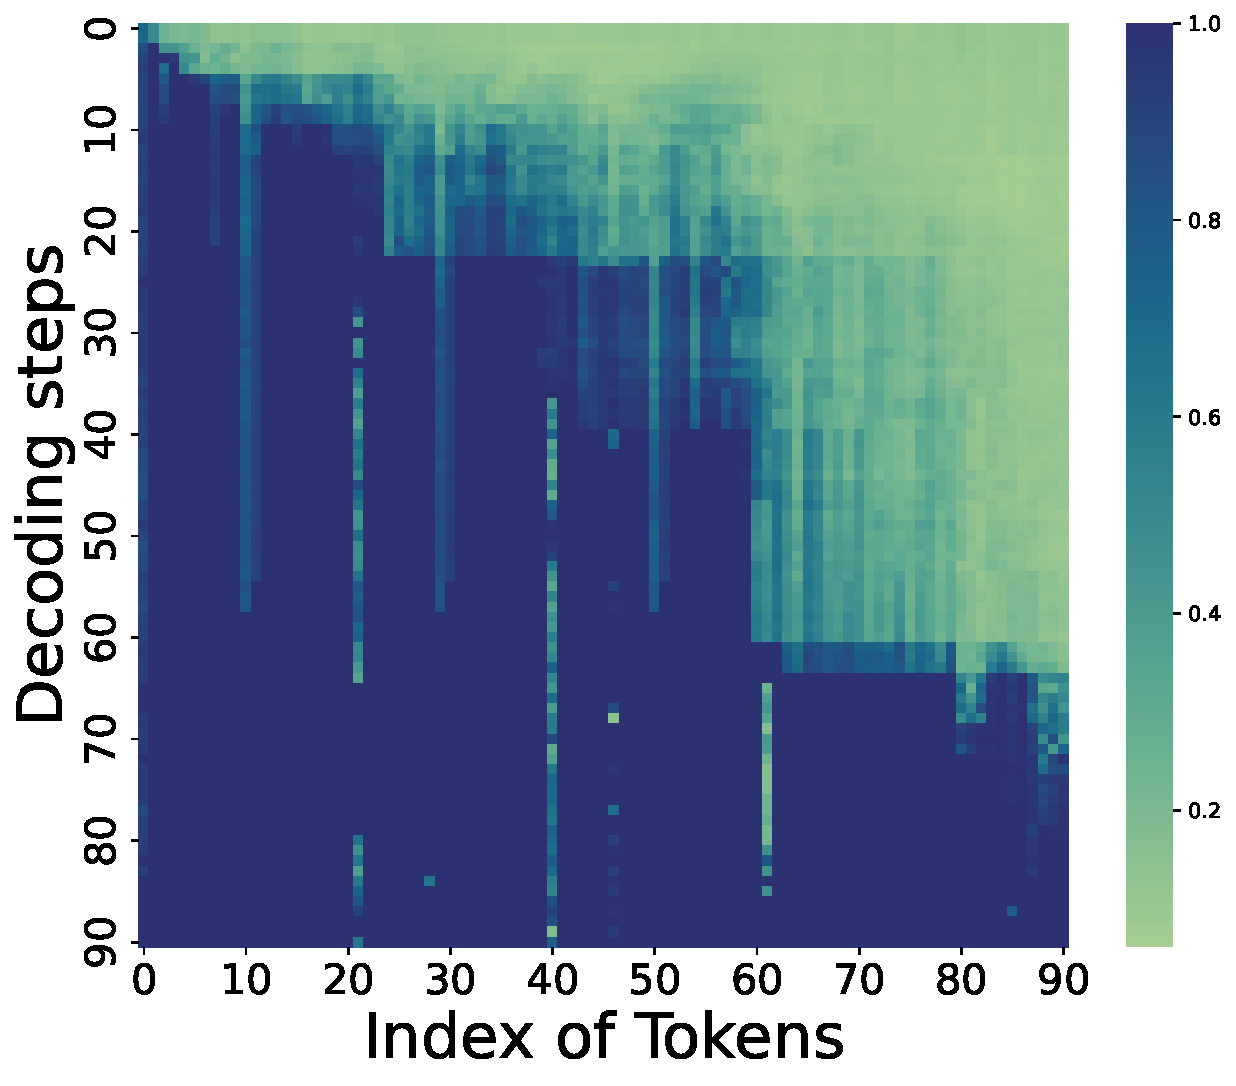
\includegraphics[width=\linewidth]{fig/heatmap3.pdf}
  \end{subfigure}
  \caption{Visualization of the decoding entropy for random samples. The x-axis is the index of generated token, while y-axis refers to decoding steps. Here we set the diffusion timestep and generation length to be equal.}
  \label{fig:appx-entropy}
\end{figure}

\subsection{Decoding Samples}
\label{sec:appx:samples}
Figure~\ref{fig:cases} demonstrates the generation order for different temperatures. The background color runs monotonically from red (earliest) through the spectrum to purple (latest). 
As we can see, the higher temperature leads to less AR sequence generation. The model tends to determine the right-hand side first, including pad tokens which decide the generation length, and the key parts of this code snippet are generated near the end.
\begin{figure}[ht]
  \centering
  \begin{subfigure}[c]{0.49\textwidth}
    \centering
    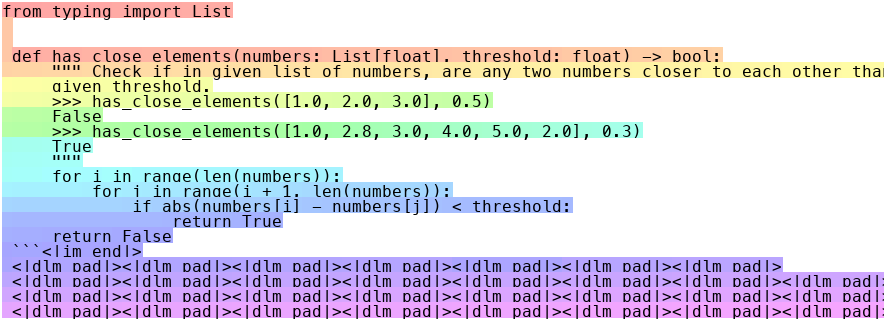
\includegraphics[width=\linewidth]{fig/case1.png}
  \end{subfigure}
  \hfill
  \begin{subfigure}[c]{0.49\textwidth}
    \centering
    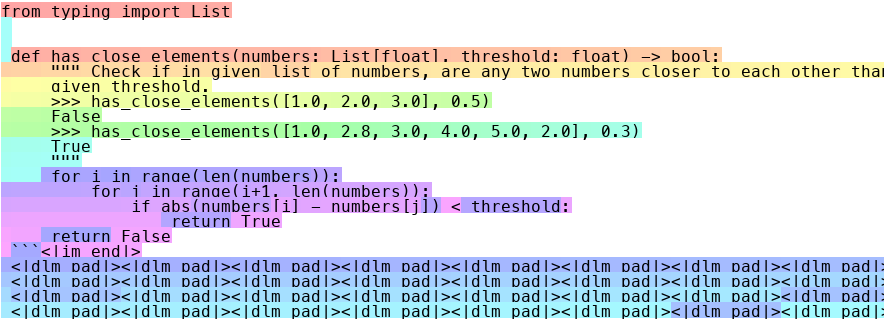
\includegraphics[width=\linewidth]{fig/case2.png}
  \end{subfigure}
  \hfill
    \begin{subfigure}[c]{0.49\textwidth}
    \centering
    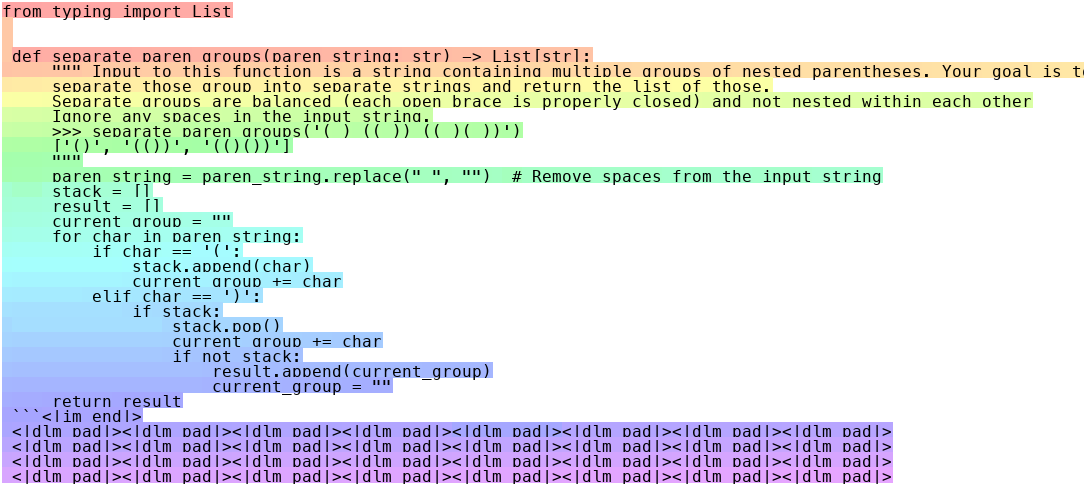
\includegraphics[width=\linewidth]{fig/case3.png}
  \end{subfigure}
  \hfill
  \begin{subfigure}[c]{0.49\textwidth}
    \centering
    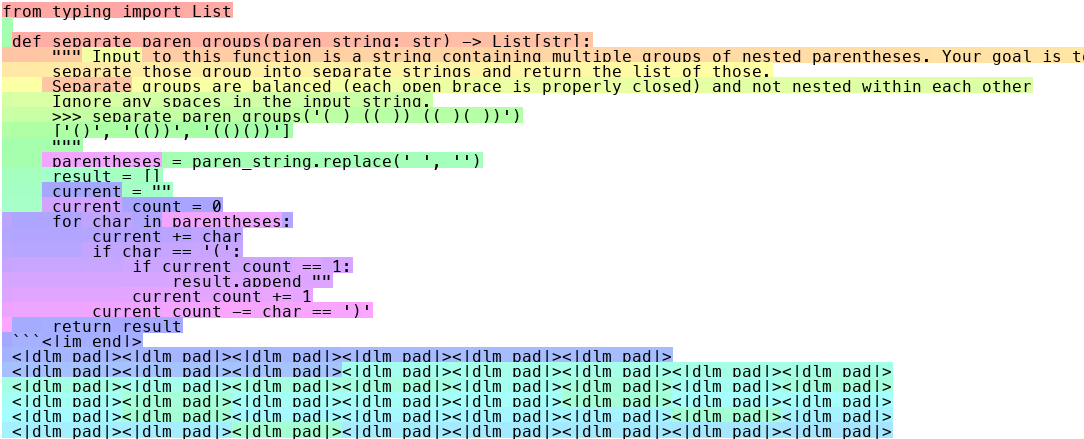
\includegraphics[width=\linewidth]{fig/case4.png}
  \end{subfigure}
  
  \caption{Visualization of the decoding trajectory of DiffuCoder-Instruct under different sampling temperatures.
Each character's background is colored from red to purple according to the recover order of the \mask. \textbf{Left}: temperature is $0.2$; \textbf{Right}: temperature is $1.2$.}
  \label{fig:cases}
\end{figure}

\subsection{Decoding Timesteps}
\begin{figure}
    \centering
    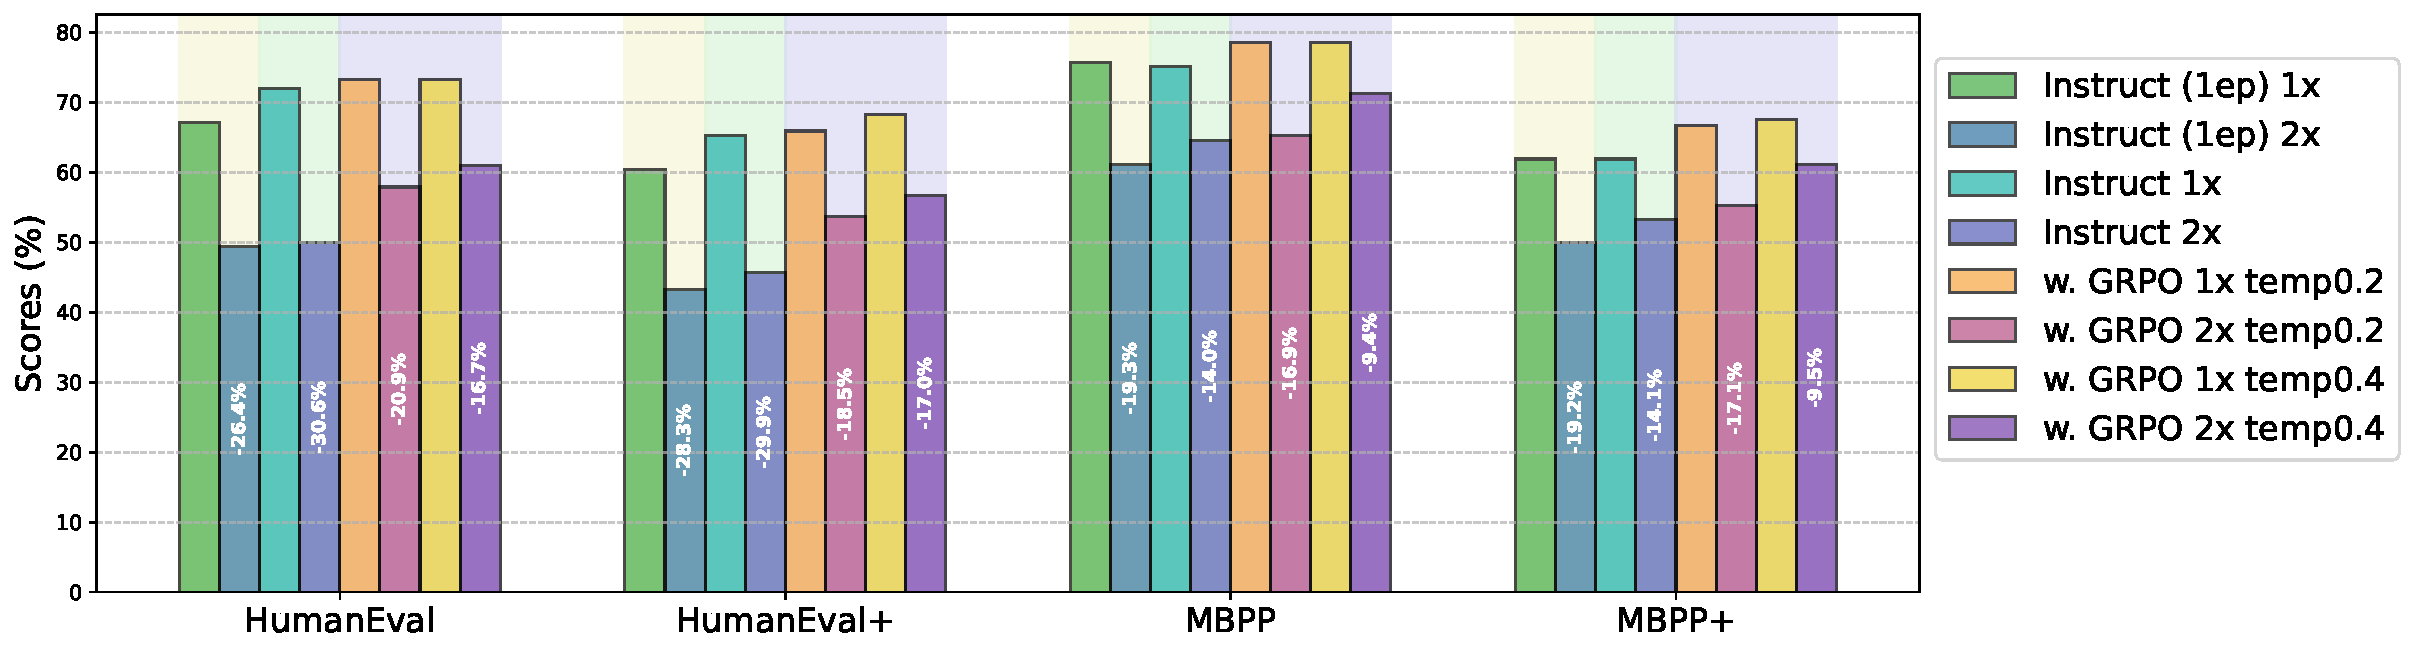
\includegraphics[width=0.99\linewidth]{fig/model_performance_comparison.pdf}
    \caption{Different model variants act differently when changing decoding timesteps to 1/2 of the sequence length. 1x means the default setting where decoding timesteps are equal to the sequence length while 2x means 1/2 fewer steps which will result in 2x speedup.}
    \label{fig:decodet}
\end{figure}
\label{sec:appx:decodet}
Another key motivation for measuring AR-ness is its relationship with generation parallelism. 
A model with very high AR-ness implies strong left-to-right token dependencies, which limits opportunities for parallel decoding. 
Conversely, lower AR-ness suggests that the model can generate multiple tokens more independently, enabling fewer diffusion steps and thus faster generation. 
In other words, by monitoring AR-ness, we also uncover how much headroom remains for accelerated, parallel decoding schedules. In Figure~\ref{fig:decodet}, if we correlate the performance drop from 1x to 2x with the non-AR (parallelism) decoding pattern, where a higher drop indicates higher AR-ness, then we can draw the following conclusions. (1) Compared with the Instruct model (the starting point of RL training), GRPO training improves DiffuCoder-Instruct's parallelism. (2) Compared with one epoch of instruction tuning, training for more epochs (5ep here) can reduce the AR-ness of the model. (3) For different sampling temperatures in the GRPO-trained DiffuCoder, the higher temperature (0.4) brings less AR-ness and thus a smaller performance drop at 2x speed.

\subsection{Coupled GRPO Training}
\label{sec:appx:grpotrain}
We monitored the completion length during GRPO training but did not observe a consistent increase in length as seen in AR GRPO training~\citep{shao2024deepseekmath,openr1}. A possible reason is that we do not encourage long-chain reasoning generation~\citep{liu2025acereason}, which could be a future research direction.

In our experimental environment, the end-to-end GRPO training time for DiffuCoder is twice that of the AR model Qwen2.5-Coder. 

\begin{figure}[ht]
  \centering
  \begin{subfigure}[c]{0.32\textwidth}
    \centering
    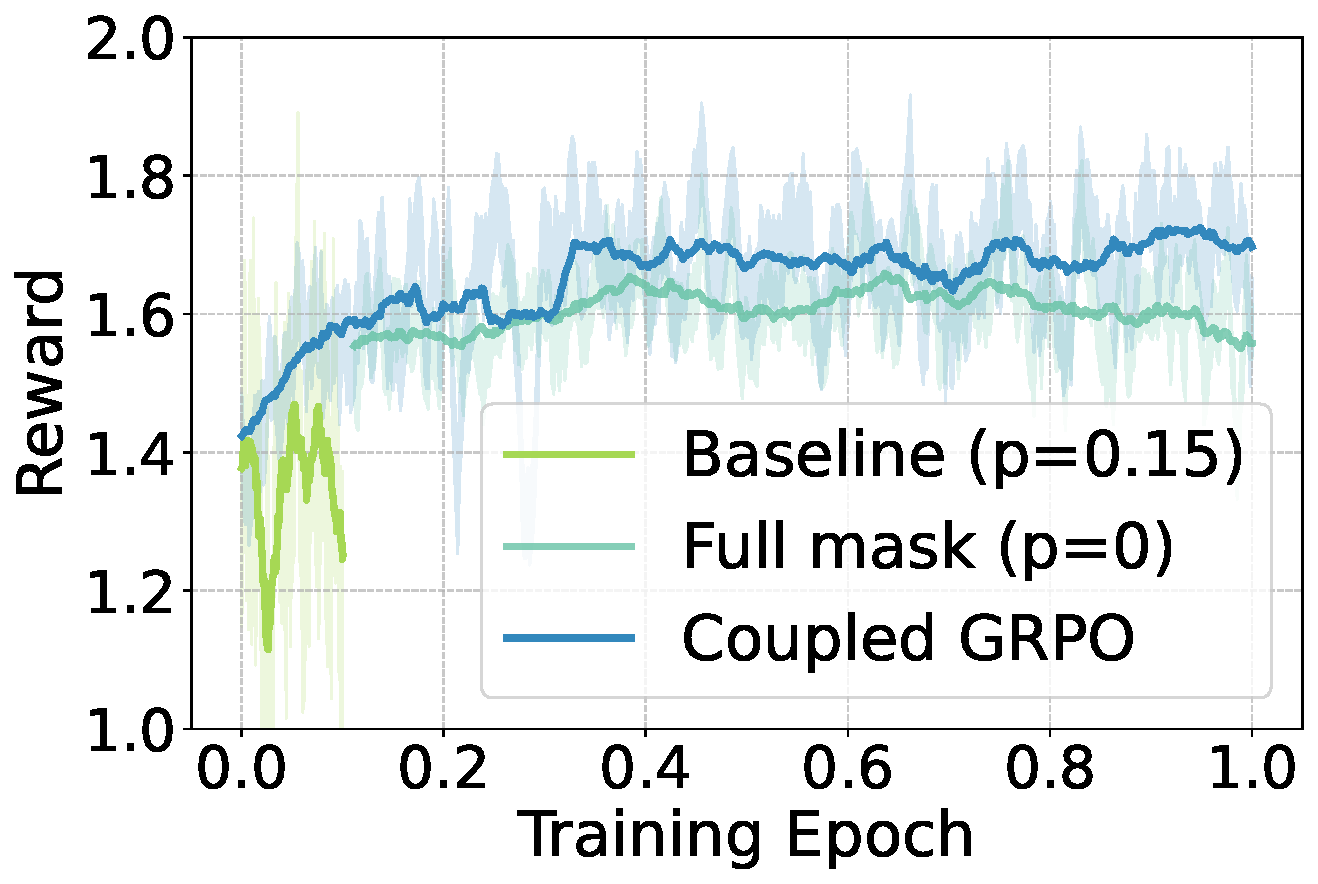
\includegraphics[width=\linewidth]{fig/reward_curves_d1.pdf}
  \end{subfigure}
  \hfill
  \begin{subfigure}[c]{0.32\textwidth}
    \centering
    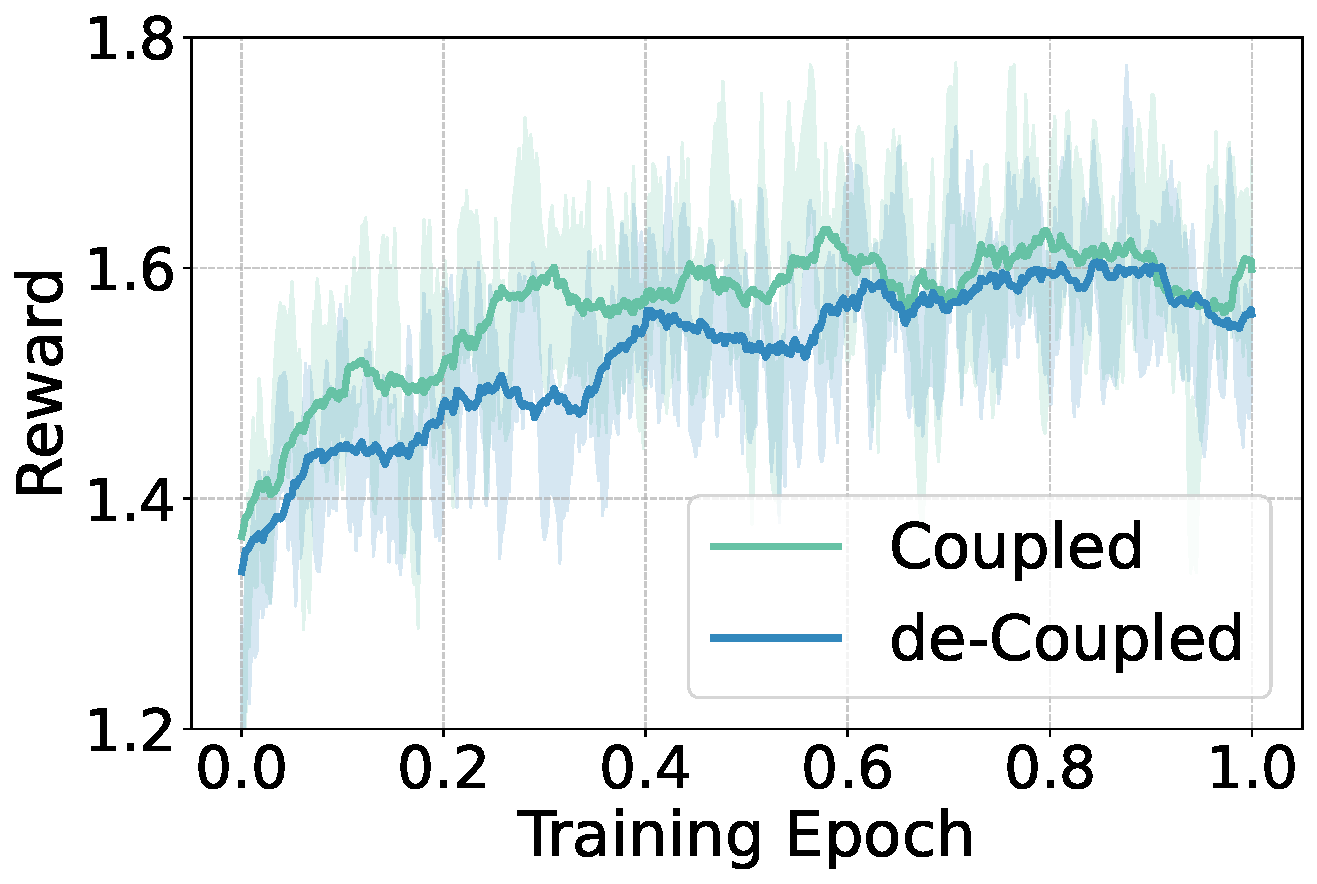
\includegraphics[width=\linewidth]{fig/reward_curves_cp.pdf}
  \end{subfigure}
  \hfill
  \begin{subfigure}[c]{0.32\textwidth}
    \centering
    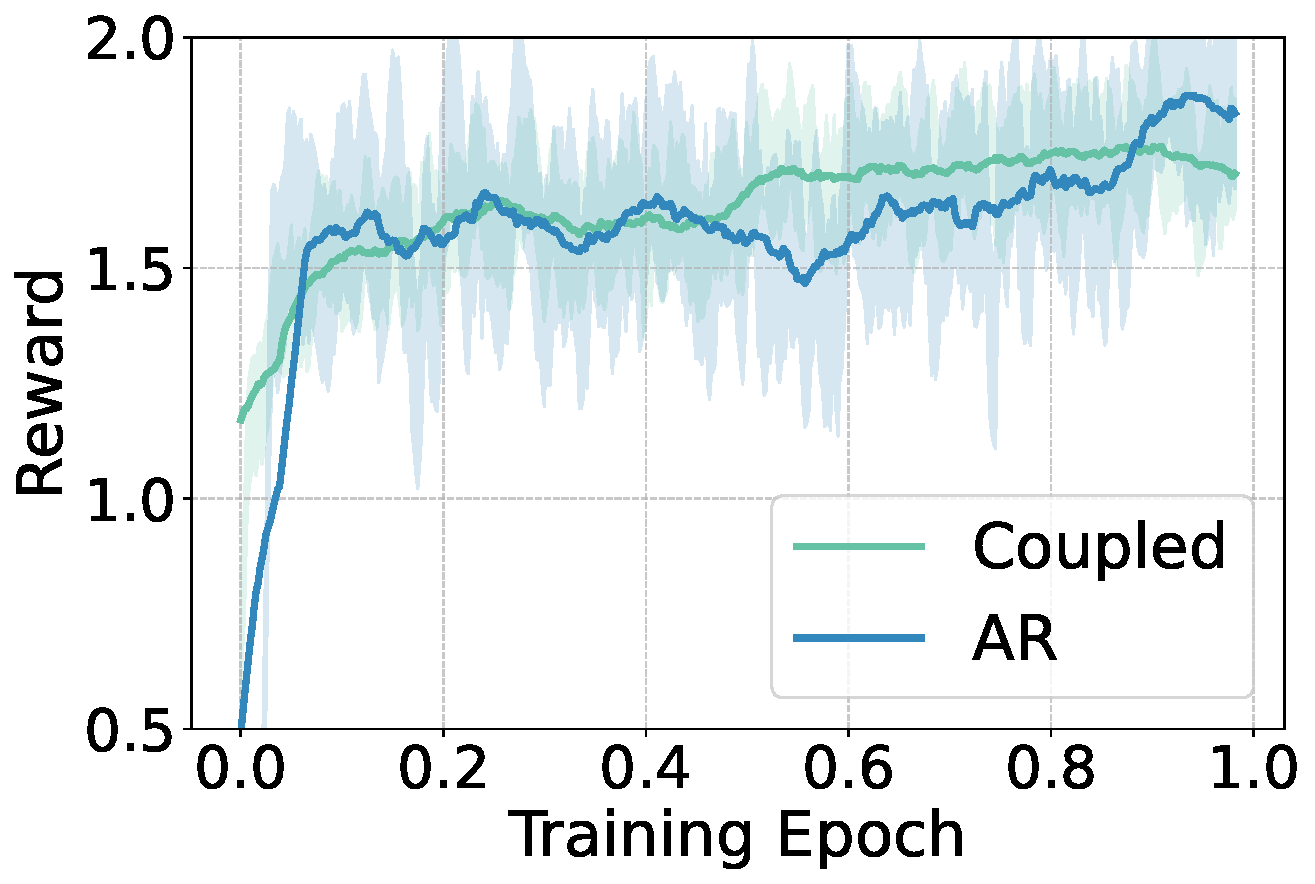
\includegraphics[width=\linewidth]{fig/reward_curves_ar.pdf}
  \end{subfigure}
  \caption{Reward curves during GRPO training. \textbf{Left}: Comparison between coupled GRPO and d1 baselines (based on an early version of DiffuCoder-Instruct). \textbf{Middle}: Decoupled GRPO uses the same number of sampling times but with randomly sampled masks (based on an early version of DiffuCoder-Instruct). \textbf{Right}: Coupled-GRPO on DiffuCoder is compared with regular GRPO for the AR model Qwen2.5Coder+SFT.}
  \label{fig:grpo-compare2}
\end{figure}

\section{Discussions}
\label{sec:appx:discuss}
\paragraph{Data Quality}
It is well-known that data quality plays a crucial role in LLM training~\citep{hui2024qwen2}. Our current experiments rely entirely on open-source community datasets~\citep{huang2024opencoder}. Since our focus is on experimental validation rather than achieving absolute performance, the data used may not be of the highest quality, and the amount of high-quality data is also limited. Future scaling, either in pre-training or RL, could benefit from better-curated datasets.

\paragraph{Template Sensitivity}
The instruction templates used in our GRPO training data~\citep{zeng2025acecoder} are relatively fixed and lack diversity. This may limit the model's generalization ability, as it could become overly reliant on specific prompt formats. Incorporating more diverse, high-quality instructions could help improve robustness during evaluation.

\paragraph{Python Code}
Our current training and evaluation primarily focus on Python. Extending these methods to multiple programming languages and exploring mixed text-code agent settings~\citep{xu2024lemur} are promising future directions.

\paragraph{Long Reasoning}
DiffuCoder has not been trained on tasks involving long reasoning chains~\citep{Polaris2025,liu2025acereason}. This is mainly due to the limited sequence length and slower inference speed of current dLLMs. Supporting longer reasoning chain remains a challenge for future work.

\paragraph{Entropy Analysis}
Recent studies on AR LLMs have examined token-level entropy changes during RL training~\citep{cui2025entropy,liu2025prorl,agarwal2025unreasonable}. A promising direction would be to further analyze token entropy in our setting to better understand its dynamics and potential impact on reward optimization.
